\documentclass[12pt]{report}
\usepackage{flushend}
\usepackage{graphicx}
\usepackage[noadjust]{cite}
% \usepackage[toc,acronym,description,sort=def]{glossaries}
\usepackage[toc,acronym,sort=def]{glossaries}
\usepackage{sectsty}
\usepackage{setspace}
\usepackage{enumerate}
\usepackage{IEEEtrantools}
\usepackage{paralist}
\usepackage{chngcntr}
\usepackage{ftnxtra}
\usepackage{amsmath}
\usepackage{algorithm}
\usepackage[noend]{algpseudocode}
\counterwithout{footnote}{chapter}
%\usepackage[top=1.4 in]{geometry}
\algnewcommand{\LeftComment}[1]{\Statex \(\triangleright\) #1}
\renewcommand{\bibname}{References}
\renewcommand{\algorithmicrequire}{\textbf{Input:}}
\renewcommand{\algorithmicensure}{\textbf{Output:}}
\chapterfont{\centering}
\pagestyle{headings}
\onehalfspacing

%************Glossary*************%

\makeglossaries

\newglossaryentry{dna}
{
    name=DNA,
    description={Deoxyribo Nucleic Acid, a molecule that codes genetic instructions in living organisms. It is a \emph{string} of 4 `nucleotides' - Nitrogen containing bases: Cytosine (C), Guanine (G), Adenine (A), and Thymine (T)}
}

 
%********End of Glossary**********%

\begin{document}

\begin{titlepage}
\begin{center}
\vspace{1cm}
\huge
\textbf{DNN Compiler for Custom AI Chip ISA}\\

\normalsize
\textbf{CS4099 Project Final Report}\\
\vspace{1cm}
\emph{Submitted by}\\        
\vspace{0.5cm}
\begin{tabular}{ccc}
\textbf{Mohammed Ameen }&& \textbf{B210515CS}\\
\textbf{Vivek K P}&& \textbf{B210473CS}\\
\textbf{Adil Abdul Jabbar}&&\textbf{B210461CS} \\
%\textbf{Name4}&&\textbf{Reg No: 4} \\
\end{tabular}\\
\vspace{0.8cm}
\textbf{Under the Guidance of\\Dr. Nirmal Kumar Boran}\\
\vspace{0.8cm}
\begin{center}
 
\includegraphics[width=0.2\textwidth]{nitc-logo.png}
\end{center}
\vspace{0.8cm}
\textbf{Department of Computer Science and Engineering}\\
\textbf{National Institute of Technology Calicut}\\
\textbf{Calicut, Kerala, India - 673 601}\\
\vspace{0.8cm}
\textbf{April 15, 2025}
\end{center}
\end{titlepage}
\pagenumbering{roman}
\begin{spacing}{1.01}
{
\thispagestyle{empty}

\fontsize{14}{14}\selectfont
\centering{\MakeUppercase{\textbf{National Institute of Technology Calicut, Kerala, India - 673 601}}} \\
\vspace*{0.5cm}
\fontsize{12}{12}\selectfont
\centering{\MakeUppercase{\textbf{DEPARTMENT OF COMPUTER SCIENCE AND ENGINEERING}}} \\
\begin{figure}[ht]
{\centering {
\includegraphics[width=0.2\textwidth]{nitc-logo.png}}\par}
\end{figure}
2025\\
\vspace{0.5cm}
\fontsize{14}{14}\selectfont
\textbf{\centering{CERTIFICATE}}\\
\vspace{0.25cm}
\fontsize{12}{12}\selectfont
\onehalfspacing{\textit{Certified that this is a bonafide record of the project work titled}}\\
\vspace*{0.25cm}
\textbf{\MakeUppercase{DNN Compiler for Custom AI Chip ISA}}\\
\vspace*{0.25cm}
\onehalfspacing{\centering{\textit{done by}}}\\
\vspace*{0.25cm}
\begin{tabular}{ccc}
\textbf{Mohammed Ameen }\\
\textbf{Vivek K P}\\
\textbf{Adil Abdul Jabbar}\\
%\textbf{Name4} \\
\end{tabular}\\
\vspace*{0.25cm}
\onehalfspacing{ \textit{\centering{of eighth semester B. Tech in partial fulfillment of the requirements for the award of the degree of Bachelor of Technology in Computer Science and Engineering of the National Institute of Technology Calicut}}}\\
\vspace*{0.5cm}
\noindent{
\begin{tabular}{p{4.8cm}cp{4.5cm}}
\textbf{Project Guide}  & \hfill \textbf{Head of Department} \\
Dr. Nirmal Kumar Boran & \hfill Dr. Subashini R\\
Assistant Professor & \hspace{5cm} Associate Professor\\
 & & \\
 & & \\
  & & \\

\end{tabular}
}
}
\chapter*{DECLARATION}
We hereby declare that the project titled, \textbf{DNN Compiler for Custom AI Chip ISA}, is our own work and that, to the best of our knowledge and belief, it contains no material previously published or written by another person nor material which has been accepted for the award of any other degree or diploma of the university or any other institute of higher learning, except where due acknowledgement and reference has been made in the text.\\

\vspace{1.2cm}

\noindent{
\begin{tabular}{p{8cm}p{6cm}}
Place : Kattangal& \\
Date :  05/05/2025& \\
\end{tabular}
}

\vspace{2cm}

\noindent{
\begin{tabular}{p{8cm}p{6cm}}
Name : Mohammed Ameen & Signature : \\
Reg. No. : B210515CS & \\
\end{tabular}
}

\vspace{1.2cm}

\noindent{
\begin{tabular}{p{8cm}p{6cm}}
Name : Vivek K P & Signature : \\
Reg. No. : B210473CS & \\
\end{tabular}
}

\vspace{1.2cm}

\noindent{
\begin{tabular}{p{8cm}p{6cm}}
Name : Adil Abdul Jabbar & Signature : \\
Reg. No. : B210461CS & \\
\end{tabular}
}

\newpage


\begin{abstract}
Our project focuses on developing a DNN compiler that translates deep neural network models from Python-based AI frameworks to a custom AI chip’s Instruction Set Architecture (ISA), designed by the \textbf{Indian Space Research Organization (ISRO)}. The compiler converts models, built and trained using libraries like TensorFlow and PyTorch, into optimized machine instructions executed by the custom ASIC

The ASIC features a CISC-style ISA, capable of performing neural network operations like convolution and pooling with just a few instructions. The compiler is responsible for extracting layer-wise information, generating instructions for each layer, managing data dependencies, and optimizing memory usage. It also handles weight extraction, preprocessing, and memory arrangement to match the chip’s expectations.

This project contributes to ISRO’s larger vision of deploying custom ASICs in future space missions for tasks like real-time image processing and AI inference, where such chips outperform conventional GPUs under strict constraints like power limitations and harsh environments.

\end{abstract}
\chapter*{\rm \large \bf ACKNOWLEDGEMENT}
It is with immense gratitude that we acknowledge the support and guidance received from several individuals, without whom the successful completion of this project would not have been possible.

First and foremost, we would like to express our sincere thanks to \textbf{Dr. Nirmal Kumar Boran}, our project guide, for his invaluable encouragement, continuous support, and insightful guidance throughout the course of this work. His expertise and mentorship played a pivotal role in shaping the direction and outcome of our project.

We extend our heartfelt appreciation to \textbf{Piyush} and \textbf{Kaustubh} from \textbf{URSC, ISRO}, key members of the ASIC chip development team, for their constant coordination, technical insights, and unwavering support in integrating our compiler with the hardware development process.

Finally, we thank all faculty members, peers, and family members who have directly or indirectly supported and encouraged us during this project.
\vspace{4.0mm}
\tableofcontents
\addtocontents{toc}{\vskip-30pt}
\end{spacing}
\listoffigures
% \listoftables
\vspace{-2 em}
\printglossary[nonumberlist]


\pagenumbering{arabic}

\chapter{Introduction}

Artificial Intelligence (AI) has emerged as a transformative technology in space exploration, enabling autonomous decision-making for complex tasks such as satellite image analysis, planetary rover navigation, and real-time sensor data processing. Among AI techniques, \textbf{Deep Neural Networks (DNNs)} have demonstrated state-of-the-art performance in domains like image classification, object detection, and time-series analysis. DNNs are structured as layered computational graphs—comprising convolutional, pooling, and fully connected layers—that extract hierarchical features from raw inputs via iterative training.

Despite their advantages, the deployment of AI models in space environments is constrained by several critical factors: \textbf{power consumption, physical size, weight, and radiation tolerance}. Conventional inference platforms, such as general-purpose GPUs, are unsuitable for space missions due to their high energy demands and limited environmental robustness. These limitations necessitate the development of specialized, low-power hardware accelerators tailored to the rigors of space-based deployment.

To address this challenge, the \textbf{Indian Space Research Organization (ISRO)} is developing a custom \textbf{Application-Specific Integrated Circuit (ASIC)} designed specifically for DNN inference in space. This ASIC is engineered to efficiently execute fundamental neural network operations—including convolution, pooling, and dense layer computation—while minimizing power usage. The ASIC leverages a \textbf{Complex Instruction Set Computing (CISC)}-style \textbf{Instruction Set Architecture (ISA)}, purpose-built to execute DNN workloads using compact and optimized instruction sequences.

\section{System Overview}
The overall inference process is coordinated by a dedicated \textbf{master processor}, which is responsible for initializing the ASIC by loading data and parameters into the appropriate \textbf{frame and filter memory} regions in RAM. The master processor orchestrates the transfer of input feature maps, kernel weights, and DSP parameters, and then triggers execution on the ASIC via control signals. This architecture ensures energy-efficient inference execution that adheres to the strict reliability and operational constraints of space missions.

This work focuses on the development of the supporting \textbf{software toolchain} required to interface with the ASIC, with particular emphasis on the design of a dedicated \textbf{DNN compiler}. This compiler serves as the bridge between high-level AI models and the ASIC's custom ISA, enabling efficient, real-time AI inference tailored for ISRO's future spaceborne platforms. The subsequent chapters will explore the system design, compiler architecture, implementation strategy, and performance evaluation in detail.

\begin{figure}[!b]
\centering
  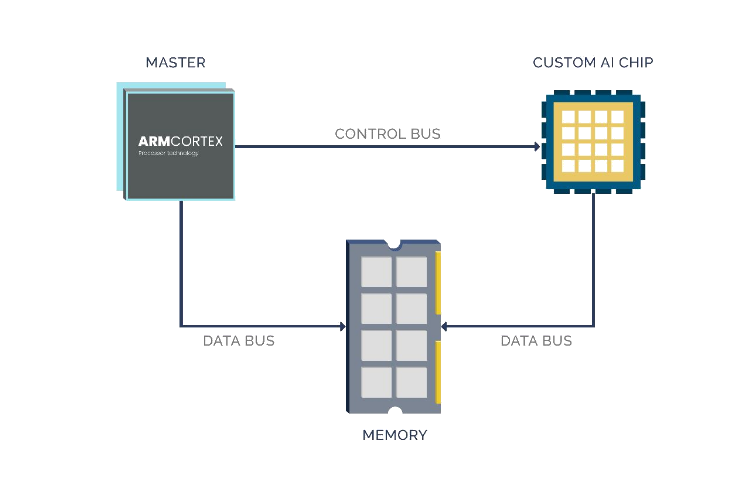
\includegraphics[width=\textwidth]{system_overview1.png}
  \caption{Diagram depicting the connection between between master processor and the AI chip.}
  \label{label5}
\end{figure}


\begin{figure}[!b]
\centering
  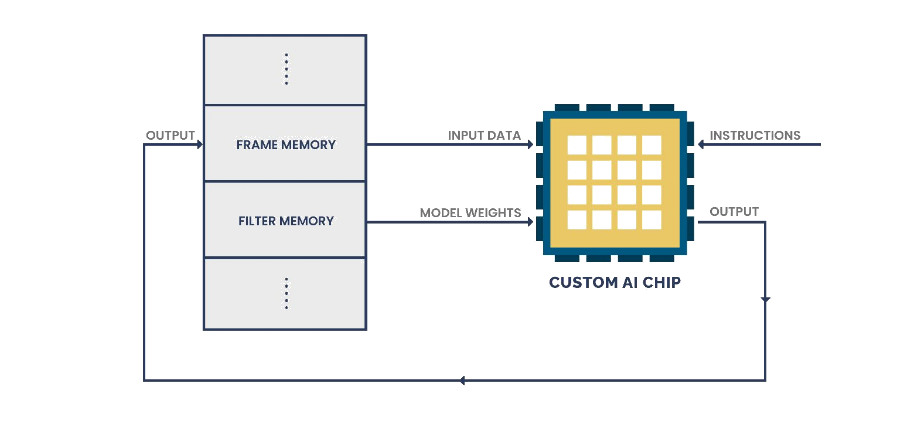
\includegraphics[width=\textwidth]{asic_data_flow1.png}
  \caption{Overview of the ASIC AI Chip}
  \label{label3}
\end{figure}


\section{Supported Layers}

The hardware provides native support for:
\begin{itemize}
    \item \textbf{Convolution layer}
    \item \textbf{Maxpooling layer}
    \item \textbf{Dense (Fully Connected) layer}
\end{itemize}

\noindent Additionally, it implicitly supports:
\begin{itemize}
    \item \textbf{Batch Normalization layer} — integrated into convolution instructions using DSP parameters (see Section~\ref{sec:dsp_parameters}).
\end{itemize}

\section{Memory Layout}

The ASIC is connected to a unified physical RAM that stores all tensors, weights, and parameters. The ISA defines two distinct virtual memory regions:

\begin{itemize}
    \item \textbf{Frame Memory}: stores input data, intermediate activations, and final outputs.
    \item \textbf{Filter Memory}: stores layer weights, DSP parameters, bias vectors and intermediate split results.
\end{itemize}

Although both memory types reside at arbitrary locations in RAM, the ISA treats each as starting from address 0.

\subsection{Frame Memory}

Frame memory holds input tensors and is updated dynamically during inference with layer-wise outputs. It is initialized using:

\subsection{Filter Memory}

Filter memory is divided into two sections:

\begin{itemize}
    \item \textbf{Weights}: Convolution filters, dense layer weights, and maxpooling placeholders.
    \item \textbf{Parameters}: DSP parameters and bias vectors.
\end{itemize}

\subsection{Data Representation}
In the ASIC’s memory layout, data is organized in a \textbf{channel-major} format:

\begin{itemize}
    \item \textbf{For tensors:} \texttt{channel} $\rightarrow$ \texttt{height} $\rightarrow$ \texttt{width}
    \item \textbf{For filters:} \texttt{filter} $\rightarrow$ \texttt{channel} $\rightarrow$ \texttt{height} $\rightarrow$ \texttt{width}
\end{itemize}

This means that all data for a given channel is stored \textit{row by row} before moving to the next channel.

\section{DSP Parameters}

The hardware supports a fused operation using three \textbf{DSP parameters} per output channel: $v_1$, $v_2$, and $v_3$. This enables bias addition and batch normalization through a single transformation, applied as:

\[
y = v_2 + v_1 \cdot (x + v_3)
\]

\begin{itemize}
    \item $x$: Intermediate value after weighted summation.
    \item $y$: Final output after applying DSP transformation.
\end{itemize}

\section{Zero Padding}

Unlike Python frameworks, the ASIC requires input tensors to be \textbf{pre-padded with zeros}. Therefore, zero-padding parameters for a given layer are associated with its \textbf{preceding layer}.

During execution, the chip automatically applies the specified padding to the preceding layer's output before it is consumed by the current layer.

\section{Supported Activation Functions}

The hardware supports the following activation functions:
\begin{itemize}
    \item \textbf{Linear} (no activation)
    \item \textbf{ReLU}
    \item \textbf{Leaky ReLU}
\end{itemize}

\noindent ReLU and Leaky ReLU are implemented via a unified operation:
\begin{verbatim}
if x < v1:
  y = v2 * x
else:
  y = x
\end{verbatim}

\noindent where $v1$ and $v2$ are configurable parameters.

\chapter{Literature Survey}

The development of efficient AI compilers for specialized hardware has emerged as a critical research area at the intersection of computer architecture and deep learning. This chapter systematically examines prior work across three key domains relevant to our project, analyzing both the strengths and limitations of existing approaches while identifying the unique contributions of our work in the context of space-grade AI acceleration.

\section{Hardware Accelerators for Space Applications}
Recent advancements in space-grade AI hardware have revealed a clear trajectory toward specialized architectures. NASA's pioneering work on radiation-hardened FPGA implementations \cite{nasa2020} demonstrated a 40% power reduction compared to conventional GPU solutions, though at the cost of limited programmability. The European Space Agency's comprehensive studies on ASIC-based vision processors \cite{esa2021} established the fundamental importance of custom instruction set architectures in achieving the dual objectives of energy efficiency and fault tolerance. Building upon these international efforts, ISRO's preliminary research on the target ASIC architecture \cite{isro2022} has shown promising performance-per-watt metrics for basic convolutional neural network operations. These collective findings strongly suggest that custom ASICs with specialized ISAs represent the most viable solution for space applications, albeit with the significant challenge of requiring sophisticated compiler support to fully realize their potential.

\section{DNN Compiler Architectures}
The landscape of DNN compiler architectures presents diverse approaches to bridging high-level models with hardware implementations. The TVM framework \cite{tvm2018} introduced a groundbreaking modular stack architecture capable of supporting multiple hardware backends, though its general-purpose design lacks specific optimizations for space applications. MLIR \cite{mlir2020} advanced the field through its innovative intermediate representation, offering unprecedented flexibility at the cost of some overhead that may be prohibitive in resource-constrained environments. Perhaps most instructive for our work, Google's EdgeTPU compiler \cite{googletpu2019} demonstrated the substantial benefits of hardware-aware optimizations, achieving threefold efficiency improvements over generic solutions. These architectural paradigms have significantly informed our compiler design while necessitating novel adaptations to meet the unique demands of space-grade hardware.

\section{Memory Optimization Techniques}
The memory architecture of our target ASIC demands particularly innovative optimization strategies. Recent research on systolic array implementations \cite{systolic2021} has shown that meticulous dataflow management can reduce memory bandwidth requirements by up to 60%, a finding that directly influenced our approach to memory hierarchy design. Weight encoding techniques \cite{encoding2020} have demonstrated the feasibility of 4:1 compression ratios for CNN filters while maintaining acceptable accuracy thresholds, suggesting promising directions for future optimization. The double-buffering methodology \cite{buffering2019} has proven particularly valuable for real-time systems, providing effective latency hiding that we have adapted for our frame memory management. These collective insights have fundamentally shaped our compiler's memory optimization strategy, especially in handling the dual memory hierarchy of frame and filter memories.

\section{Gaps Addressed by Our Work}
The comprehensive review of existing literature reveals several critical gaps that our work specifically addresses. Most notably, no prior compiler solution supports the distinctive CISC-style ISA implemented in ISRO's space-grade ASIC, creating a fundamental incompatibility with existing toolchains. Furthermore, current frameworks lack support for the computation splitting paradigm required by the ASIC's limited processing elements, a constraint that demands novel compilation strategies. Our compiler architecture synthesizes the most effective elements from prior work while introducing innovative solutions tailored to space-specific constraints, as will be detailed in the subsequent chapters of this report. This dual approach of leveraging established best practices while developing targeted innovations positions our work to make unique contributions to the field of space-grade AI acceleration.
\chapter{Problem Definition}

Deep Neural Networks (DNNs) are increasingly used in space missions for tasks like image processing, autonomous navigation, and onboard decision-making. However, conventional GPU-based inference systems are unsuitable for space applications due to high power consumption, size, and lack of environmental resilience.

To address these challenges, the Indian Space Research Organization (ISRO) is developing a custom Application-Specific Integrated Circuit (ASIC) with a CISC-style Instruction Set Architecture (ISA), optimized for AI inference in harsh, resource-constrained environments. While the hardware is being developed, a major gap exists in translating trained AI models into machine instructions compatible with this ASIC.

This project aims to develop a compiler that converts models, built using Python frameworks into optimized machine code for the ASIC. The compiler handles instruction generation, memory management, and model-to-ISA mapping, enabling real-time, power-efficient AI inference on ISRO’s space missions.

\chapter{Methodology}
This section outlines the step-by-step process followed in designing and implementing the DNN compiler for the custom AI chip. The compiler serves as a bridge between Python-based AI frameworks and the custom Instruction Set Architecture (ISA) of the ASIC. The focus here is on how trained AI models and input data are transformed into machine-level instructions and memory layouts compatible with the chip's architecture. 

The compilation process is divided into three major stages: \textbf{Frame Memory Initialization}, \textbf{Filter Memory Initialization}, and \textbf{Instruction Generation}. Each of these is described in detail below.

\begin{figure}[!b]
\centering
  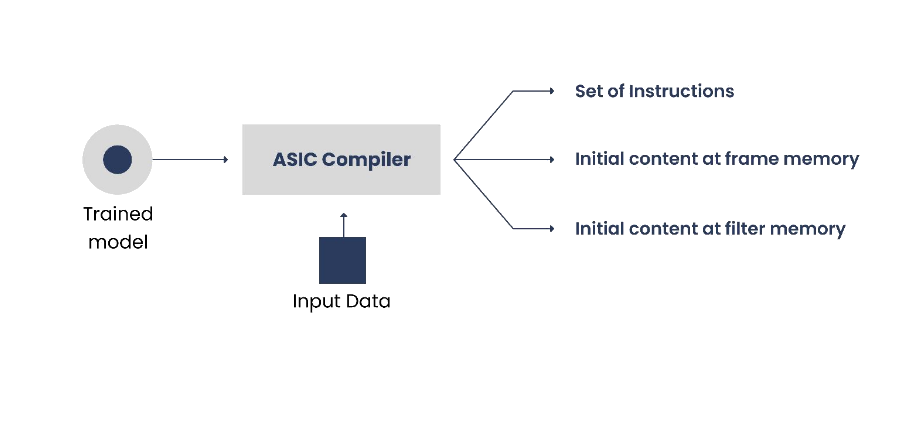
\includegraphics[width=\textwidth]{asic_dnn_compiler1.png}
  \caption{Overview of the compiler}
  \label{label1}
\end{figure}

\section{System Inputs and Outputs}

The compiler accepts two primary inputs:
\begin{itemize}
    \item A trained AI model in \texttt{H5} format, created using frameworks like TensorFlow or PyTorch.
    \item Input data, typically images or sensor data, to be processed by the model.
\end{itemize}

The outputs produced by the compiler are:
\begin{itemize}
    \item A \textbf{Frame Memory image file}, representing the initial layout of feature maps in memory.
    \item A \textbf{Filter Memory image file}, containing kernel weights, DSP parameters, and other configuration data.
    \item A sequence of \textbf{machine instructions} written in the ASIC's custom ISA, directing the chip to emulate the model.
\end{itemize}

\begin{figure}[!b]
\centering
  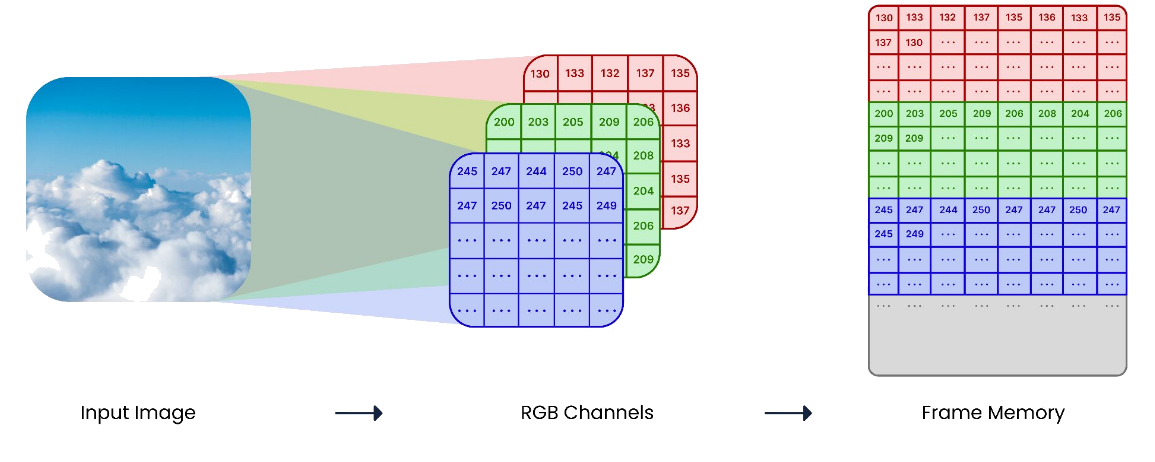
\includegraphics[width=\textwidth]{extract_ip_data1.png}
  \caption{Input extraction process for frame memory}
  \label{label4}
\end{figure}

The \textbf{master processor} is responsible for writing these memory images to their corresponding memory regions in RAM and initiating the ASIC execution.

\section{Frame Memory Initialization}

The \textbf{frame memory} is a dedicated virtual memory space used to store both input data and intermediate feature maps generated during model inference.

The compiler reads the \textit{input shape} from the trained model and reshapes the input data accordingly. If the first layer requires zero-padding, this padding is applied directly to the input before any computation. Unlike typical deep learning frameworks where padding is implicit, the ASIC expects the input tensor to be \textit{pre-padded}, meaning the padding must be present in the input written to memory.

After applying zero-padding, the data is converted into a binary format compatible with the ASIC's memory layout. This binary is written into a file that initializes the frame memory, ensuring the ASIC accesses the input in the correct padded format and memory location at the beginning of inference.

\section{Filter Memory Initialization}

The \textbf{filter memory} stores the kernel weights required by convolutional and dense layers, along with the \textbf{DSP parameters}, which optimize operations such as bias addition and batch normalization.

The compiler iterates through each relevant layer of the model, performing the following:
\begin{itemize}
    \item Extracting kernel weights and converting them into binary format.
    \item Sequentially appending these weights to the filter memory data file.
    \item Calculating and appending the corresponding DSP parameters for each operation, based on the model’s configuration.
\end{itemize}

\textbf{Special handling is required for the first Dense layer after a Flatten layer.} Since Keras uses a \textit{height $\rightarrow$ width $\rightarrow$ channel} memory order and the hardware expects a \textit{channel-major} format, the weights must be \textbf{reordered} to align with the hardware's memory layout. This ensures consistency in dot product computations during inference.


At the end of this stage, the filter memory image file contains all the necessary kernel weights and DSP parameters in the correct order for efficient access during inference.

\subsection{DSP Parameters}

The hardware supports a fused \textbf{DSP operation} using three parameters per output channel: $v_1$, $v_2$, and $v_3$. This enables both \textbf{bias addition} and \textbf{batch normalization} in a single step, applied at the \textit{instruction level}.

\textbf{Without splitting}, DSP is integrated into the convolution instruction. \textbf{With splitting}, it is applied only in the final addition instruction to ensure correctness after accumulation.

\subsection*{Parameter Computation}
\begin{itemize}
    \item With batch normalization:
    \[
    v_1 = \frac{\gamma}{\sqrt{\text{variance} + \epsilon}}, \quad
    v_2 = \beta, \quad
    v_3 = \text{bias} - \text{mean}
    \]
    \item Without batch normalization:
    \[
    v_1 = 1, \quad
    v_2 = 0, \quad
    v_3 = \text{bias}
    \]
\end{itemize}


\section{Instruction Generation}

In this stage, the compiler generates a sequence of machine instructions that direct the ASIC on how to process the model layer by layer. The compiler reads the model sequentially, and for each layer:
\begin{itemize}
    \item Extracts details such as stride, padding, kernel size, input/output addresses, and DSP parameter addresses.
    \item Generates instructions that conform to the ASIC’s CISC-style ISA, efficiently handling operations like convolution, max pooling, and dense computations.
\end{itemize}

\begin{figure}[!b]
\centering
  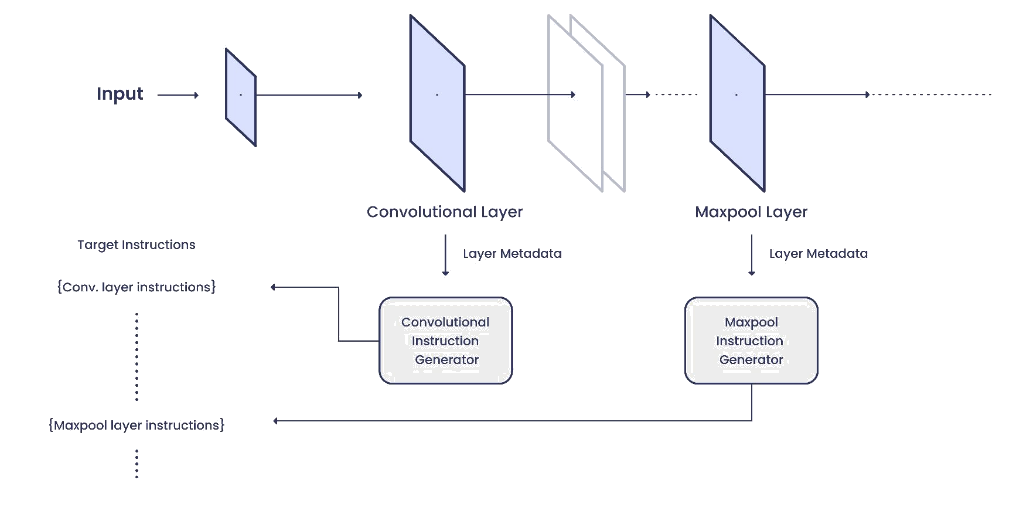
\includegraphics[width=\textwidth]{instruction_generation1.png}
  \caption{Instruction generation process}
  \label{label2}
\end{figure}

\subsection{Activation Functions}


\textbf{ReLU} and \textbf{Leaky ReLU} are implemented using a unified hardware operation:
\[
y = 
\begin{cases}
v_2 \cdot x & \text{if } x < v_1 \\
x & \text{otherwise}
\end{cases}
\]

\noindent
where $x$ is the input value, $y$ is the activated output, and:
\subsection*{Parameter Calculation}
\begin{itemize}
    \item For ReLU: $v_1 = 0$, $v_2 = 0$
    \item For Leaky ReLU: $v_1 = 0$, $v_2$ is the negative slope (e.g., $0.01$)
\end{itemize}

\section{Hardware Limitations and Splitting}

In the AI chip, the \textbf{block size} refers to the total number of input tensor elements processed together to compute a single output value. This is equivalent to the size of the convolution filter:

\[
\text{Block size} = \text{filter height} \times \text{filter width} \times \text{filter depth}
\]

This block is the smallest unit that must be computed in a single cycle. If the available parallel processing elements are fewer than the block size, the compiler automatically \textbf{splits} the convolution or dense operation into smaller sub-blocks. These partial computations are independently executed and their results are accumulated to generate the final output.

The same mechanism is applied to \textbf{Dense layers}, which are treated as a special case of convolution. However, the splitting strategy differs between convolution and dense layers based on data layout and filter structure.

\section{Summary}

This methodology outlines the complete pipeline from parsing a trained model and input data to generating machine-ready instruction sets and memory images for the ASIC chip. The seamless integration of the splitting mechanism within the instruction generation phase allows the compiler to efficiently handle models even under hardware limitations. 

The compiler ensures that frame and filter memories are properly initialized, DSP parameters are applied correctly, and the generated instruction stream executes the model reliably on ISRO’s custom AI hardware.

\chapter{Results}

To validate the correctness of the compiler outputs, multiple levels of verification were performed across memory initialization, instruction generation, and hardware inference results.

\section{Model Compatibility}

The compiler currently supports sequential deep neural network (DNN) architectures composed of convolution, batch normalization, maxpooling, and dense layers. This includes standard models such as \textbf{AlexNet}, \textbf{ResNet}, and \textbf{VGGNet}, which have been successfully compiled and verified on the hardware.

\section{Memory Verification}

For each applicable layer, kernel weights and biases were saved and inspected to ensure they are stored in the correct order and format. This step confirmed that both the \textbf{Filter Memory image} and associated metadata conformed to the expected structure defined by the ISA and compiler specifications.

\section{Instruction Verification}

Instruction correctness was verified by storing and reviewing metadata about each layer, including:
\begin{itemize}
    \item Addresses of weights, biases, and DSP parameters
    \item Input and output tensor addresses
\end{itemize}
These were cross-checked against expected values to confirm that the generated instructions correctly reference the initialized memory regions.

\section{Output Verification}

To further validate the correctness of execution, intermediate outputs from each layer were generated using a Python model that mimics the ASIC's behavior. These were then compared against the corresponding outputs from the hardware after each layer. The results consistently matched, confirming that the compiler and chip produced functionally correct outputs across all supported layers.

\chapter{Conclusion and Future Work}

\section{Conclusion}
This project has successfully developed a DNN compiler for ISRO's custom AI ASIC, enabling efficient deployment of neural networks in space-constrained environments. The compiler bridges the critical gap between high-level AI models and the ASIC's specialized architecture by:

\begin{itemize}
    \item Automatically translating trained models (TensorFlow/PyTorch) into optimized ASIC instructions
    \item Intelligently managing the ASIC's dual-memory hierarchy (frame and filter memory)
    \item Implementing computation splitting to work within hardware constraints while preserving model accuracy
\end{itemize}

Validation tests confirmed the compiler's ability to handle fundamental DNN operations (convolutional, pooling, and dense layers) while maintaining functional equivalence with reference implementations. Although the current implementation shows slower processing speeds compared to GPUs, its superior power efficiency and compact form factor make it ideally suited for space applications where energy conservation is paramount.

\section{Future Work}
To enhance the compiler's capabilities and broaden its applications, several key improvements are planned:

\subsection{Architectural Expansion}
\begin{itemize}
    \item Support for complex networks (UNet, HRNet) with skip connections
    \item Implementation of attention mechanisms for transformer-based models
\end{itemize}


\subsection{Model Format Support}
\begin{itemize}
    \item Expansion beyond current H5 support to include model formats like pth and ONNX.
\end{itemize}

\subsection{Performance Optimization}
\begin{itemize}
    \item Advanced memory allocation strategies for large-scale models
\end{itemize}

\subsection{Developer Tools}
\begin{itemize}
    \item Integrated debugging and visualization tools
    \item Profiling capabilities for power/performance analysis
\end{itemize}

\section{Final Remarks}
This compiler represents a crucial enabling technology for AI-powered space systems, demonstrating that specialized hardware-software co-design can overcome the challenges of deploying neural networks in resource-constrained environments. As both the compiler and ASIC architecture mature, they will play an increasingly important role in ISRO's autonomous space exploration initiatives.

\addcontentsline{toc}{chapter}{References}
% add BibTex of References in the project.bib file
\nocite{*}
\bibliographystyle{ieeetr}

\bibliography{project.bib}
\end{document}
